\documentclass[a4paper,margin=1in]{article}
\setlength{\columnsep}{10pt}                                                                    %兩欄模式的間距
\setlength{\columnseprule}{0pt}                                                                %兩欄模式間格線粗細

\usepackage{fullpage} % Package to use full page
\usepackage{parskip} % Package to tweak paragraph skipping
\usepackage{tikz} % Package for drawing
\usepackage{amsmath}
\usepackage{hyperref}
\usepackage{fancyhdr}	
\usepackage[CheckSingle, CJKmath]{xeCJK}
\usepackage{amsmath, courier, listings, fancyhdr, graphicx}
\setCJKmainfont{Source Han Sans TC}

\usepackage{caption}
\usepackage{subcaption}
\usepackage{placeins}

\title{線性代數作業1}
\author{0516009 吳宗達}
\date{2016/11/16}

\begin{document}
\large
\fancyhead[R]{交通大學105學年度線性代數作業}
\maketitle

\section{背景介紹}
給你 n 個點對 ($\mathit{x_{i}}$,$\mathit{y_{i}}$) 和 m 個方程式 $\mathbf{F_{k}}(x)$,找出一組係數$\widehat{x}$使得$\sum_{k=0}^{m}\mathbf{F_{k}}(x_{i})$ 與 $y_{i}$ 要盡量靠近,也就是 $e(w)$ = $\sum_{i=1}^{n}(\sum_{k=0}^{m}\mathbf{F_{k}}(x_{i})-y_{i})^2/n$ 要最小化

\section{程式說明}
以 matlab2016 來實做程式,可以到 https://github.com/cthbst/LAclass 下載本程式

\newpage
\section{執行結果}
\subsection{測試1}
以 $F_{k}(x)$=$\frac{1}{{\sqrt{2\pi}\sigma_m}}exp( \frac{-(x-\mu_{2})^2}{2\sigma_{m}^2} )$ 逼近\\ \\ \\ \\
$Dataset1$
\begin{figure}[!htbp]
	\centering
	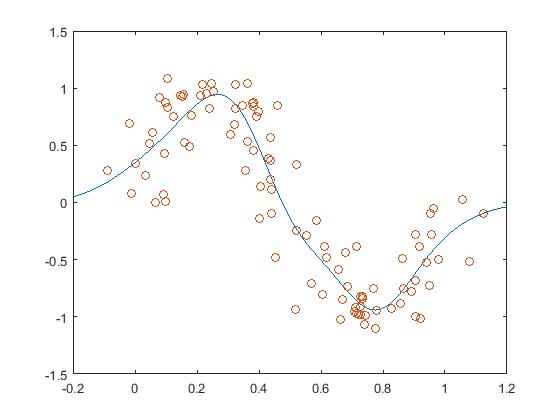
\includegraphics[width=\linewidth]{Figure11.jpg}
	\captionof{figure}{$e(w)$ = 0.0741}
\end{figure}
\newpage
$Dataset2$
\begin{figure}[!htbp]
	\centering
	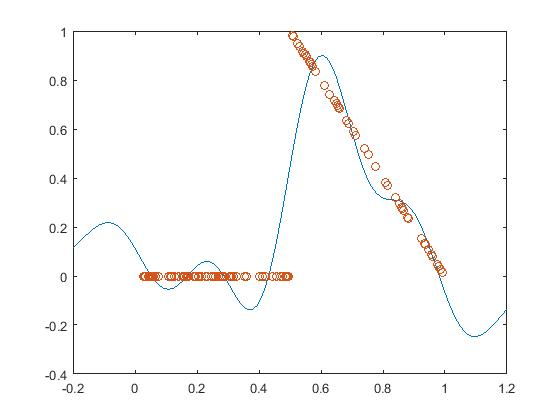
\includegraphics[width=\linewidth]{Figure12.jpg}
	\captionof{figure}{$e(w)$ = 0.0169}
\end{figure}

\newpage

\subsection{測試2}
以 $F_{k}(x)$=$x^k$ 逼近\\ \\ \\ \\ 
$Dataset1$
\begin{figure}[!htbp]
	\centering
	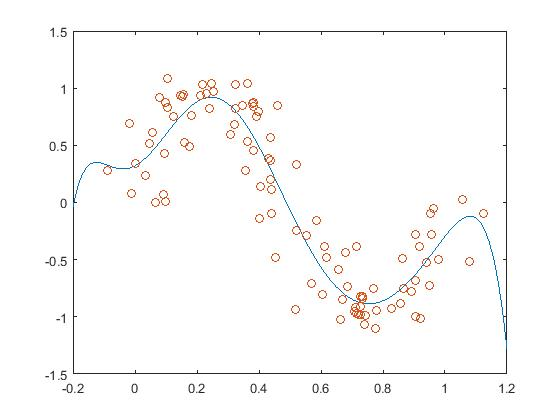
\includegraphics[width=\linewidth]{Figure21.jpg}
	\captionof{figure}{$e(w)$ = 0.0750}
\end{figure}
\newpage
$Dataset2$
\begin{figure}[!htbp]
	\centering
	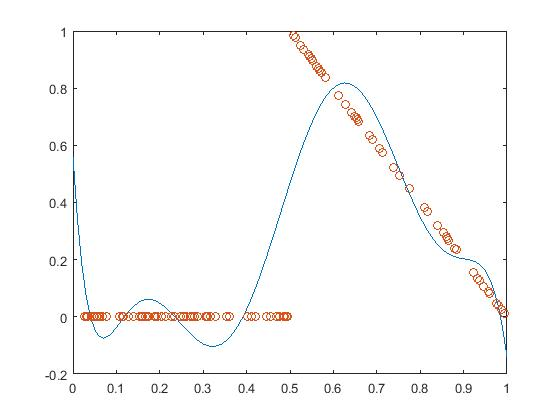
\includegraphics[width=\linewidth]{Figure22.jpg}
	\captionof{figure}{$e(w)$ = 0.0236}
\end{figure}
\newpage
\section{結論}

觀察誤差值,可以看出用鐘型曲線逼近,在 Dataset1 和 Dataset2 逼近的表現都比多項式好,以及可以看出因為 Dataset1 的資料分佈較鬆散,不同函數下可以改善的誤差值有限,而 Dataset2 資料分佈較為密集, 誤差值得差異相對大了許多。

\end{document}
